\section*{Problem No.3} \label{sec:prob3}

The following three pieces of code implements composite trapezoidal rule, composite Simpson's rule and composite 3-point Gaussian quadrature respectively. 
\begin{lstlisting}
function result = Trapezoidal(Func, n, a,b)
    %apply composite trapezoidal rule to approximate the intergation 
    %of Func between a and b using n-subintervals 
    result = Func(a)/2.0;
    h = (b-a)/n;
    for int = 1:1:n-1
        result = result + Func(a + int*h);
    end
    result = result + Func(b)/2.0;
    result =result * h;
end
\end{lstlisting}


\begin{lstlisting}
function result = Simpson(Func, n, a,b)
    %apply composite Simpson's rule to approximate the intergation 
    %of Func between a and b using n-subintervals 
    result=Func(a);
    h = (b-a)/n;
    for int =1:1:n-1
        if mod(int,2) == 0
            factor = 2;%even
        else
            factor = 4; %odd
        end
        result = result + factor * Func(a + int*h);
    end
    result = result + Func(b);
    result = result * h/3;
end
\end{lstlisting}


\begin{lstlisting}
function result = GaussianQuad(Func, n, a,b)
    %apply Gaussian Quadrature rule to approximate the intergation 
    %of Func between a and b using n-subintervals 
    result=0;    
    h = (b-a)/n;
    for int =0:1:n-1
       %for each interval apply the 3-point GQ
       myA = a + int*h;
       myB = myA + h;       
       myH = (myB-myA)/18;       
       p0 = ((myA + myB)/2.0) - sqrt(3.0/5.0)*((myB- myA)/2.0);
       p1 = ((myA + myB)/2.0);
       p2 = ((myA + myB)/2.0) + sqrt(3.0/5.0)*((myB- myA)/2.0);       
       result = result + myH*(5.0*Func(p0) + 8.0*Func(p1) + 5.0*Func(p2));       
    end
end
\end{lstlisting}


\begin{figure}[H]
 \centering
\begin{tabular}{ |c || c|c|c |}
 \hline
\#points  & Trapezoidal & Simpson's & 3-pts Guassian quad \\   	
  \hhline{|=|=|=|=|}                           
2  & 0.03564926 & 0.000579323     &	1.32050086e-08 \\
4  & 0.00894007 & 3.701346270e-05 &	2.07645012e-10 \\ 
8  & 0.00223676 & 2.326240851e-06 &	3.25006688e-12 \\
16 & 0.00055930 & 1.455928460e-07 &	5.12923037e-14 \\
32 & 0.00013983 & 9.102726350e-09 &	8.88178419e-16 \\
 \hline
\end{tabular} 
  \caption{The error of Trapezoidal rule, Simpson's rule and 3-points Guassian quadrature for evaluating $\int^{1}_{0}e^{x}.dx$ }
   \label{tab:err}
\end{figure}

The three methods were used to evaluate $\int^{1}_{0} e^{x}.dx$ using 2,4,8,16 and 32 intervals. Table \ref{tab:err} and Figure \ref{fig:p3_err_fig} show the error in numbers and on a log-log scale. The figures suggests that the Trapezoidal rule is indeed second order accurate (slope of the line is 1.99851), Simpson's rule is fourth order accurate (slope of the line is 3.98942), and the 3 points Guassian quadrature is sixth order accurate (slope of the line is 5.9564).


\begin{figure}[H]
 \centering  
   {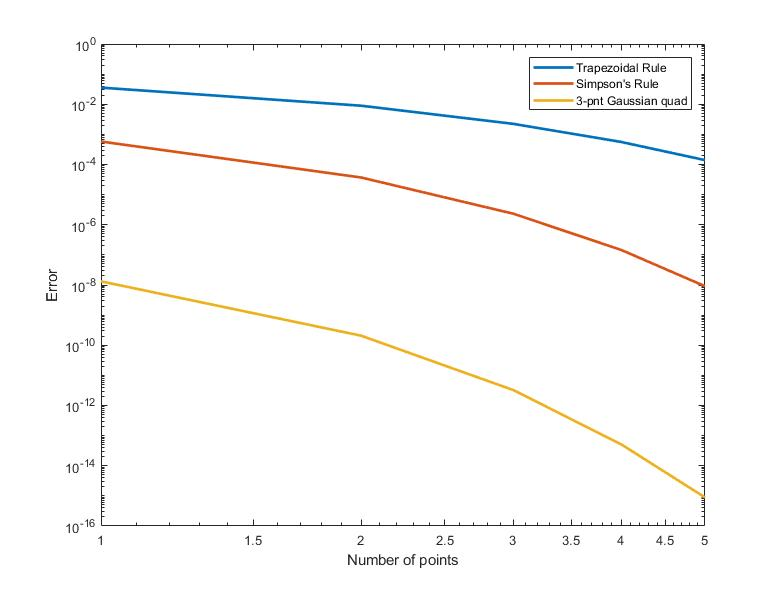
\includegraphics[width=0.7\linewidth]{fig/prob3.jpg}}   
  \caption{The log-log plot for the error for using the three integration techniques to evaluate $\int^{1}_{0} e^{x}.dx$. }
   \label{fig:p3_err_fig}
\end{figure} 
